% Template KLTN cho SV trường ĐHKHTN
% Liên hệ: nqminh@fit.hcmus.edu.vn
% Last update: 08/06/2016

% Chú ý: đọc các phần chú ý đóng khung của file này và chỉnh lại cho phù hợp.
% Trước khi build, xóa hết các file được tạo ra trong quá trình build trước đó, và build theo thứ tự: BIB > PDF > PDF.
% Nếu cập nhật tài liệu tham khảo, cũng cần build lại theo cách trên.

\documentclass[oneside,a4paper,14pt]{extreport}

% Font tiếng Việt
\usepackage[T5]{fontenc}
\usepackage[utf8]{inputenc}
\DeclareTextSymbolDefault{\DH}{T1}

% Tài liệu tham khảo
\usepackage[
	sorting=nty,
	backend=bibtex,
	defernumbers=true]{biblatex}
\usepackage[unicode]{hyperref} % Bookmark tiếng Việt
\addbibresource{References/references.bib}

\makeatletter
\def\blx@maxline{77}
\makeatother

% Chèn hình, các hình trong luận văn được để trong thư mục Images/
\usepackage{graphicx}
\graphicspath{ {Images/} }

% Chèn và định dạng mã nguồn
\usepackage{listings}
\usepackage{color}
\definecolor{codegreen}{rgb}{0,0.6,0}
\definecolor{codegray}{rgb}{0.5,0.5,0.5}
\definecolor{codepurple}{rgb}{0.58,0,0.82}
\definecolor{backcolour}{rgb}{0.95,0.95,0.92}
\lstdefinestyle{mystyle}{
    backgroundcolor=\color{backcolour},   
    commentstyle=\color{codegreen},
    keywordstyle=\color{magenta},
    numberstyle=\tiny\color{codegray},
    stringstyle=\color{codepurple},
    basicstyle=\footnotesize,
    breakatwhitespace=false,         
    breaklines=true,                 
    captionpos=b,                    
    keepspaces=true,                 
    numbers=left,                    
    numbersep=5pt,                  
    showspaces=false,                
    showstringspaces=false,
    showtabs=false,                  
    tabsize=2
}
\lstset{style=mystyle}

% Chèn và định dạng mã giả
\usepackage{amsmath}
\usepackage{algorithm}
\usepackage[noend]{algpseudocode}
\makeatletter
\def\BState{\State\hskip-\ALG@thistlm}
\makeatother

% Bảng biểu
\usepackage{multirow}
\usepackage{array}
\newcolumntype{L}[1]{>{\raggedright\let\newline\\\arraybackslash\hspace{0pt}}m{#1}}
\newcolumntype{C}[1]{>{\centering\let\newline\\\arraybackslash\hspace{0pt}}m{#1}}
\newcolumntype{R}[1]{>{\raggedleft\let\newline\\\arraybackslash\hspace{0pt}}m{#1}}



 
% Đổi tên mặc định
\renewcommand{\chaptername}{Chương}
\renewcommand{\figurename}{Hình}
\renewcommand{\tablename}{Bảng}
\renewcommand{\contentsname}{Mục lục}
\renewcommand{\listfigurename}{Danh sách hình}
\renewcommand{\listtablename}{Danh sách bảng}
\renewcommand{\appendixname}{Phụ lục}

% Định dạng chapter
\usepackage{titlesec}
\titleformat{\chapter}
    [display] 
    {\normalfont\bfseries\Large}{\chaptername \ \thechapter}{10pt}{\huge}
\titlespacing*{\chapter}{0pt}{-10pt}{40pt} %khoảng cách giữa chapter và đầu trang

\titleformat{\section}
    {\normalfont\bfseries\large}{\thesection}{1em}{}
 
\titleformat{\subsection}
    {\normalfont\bfseries\normalsize}{\thesubsection}{1em}{}
  
% Dãn dòng 1.5
\usepackage{setspace}
\onehalfspacing

% Thụt vào đầu dòng
\usepackage{indentfirst}

% Canh lề
\usepackage[
  top=20mm,
  bottom=10mm,
  left=30mm,
  right=20mm,
  footskip = 15mm,
  includefoot]{geometry}
  
% Trang bìa
\usepackage{tikz}
\usetikzlibrary{calc}
\newcommand\HRule{\rule{\textwidth}{1pt}}

% ========================================================================================= %
% CHÚ Ý: Thông tin chung về KLTN - sinh viên điền vào đây để tự động update các trang khác  %
% ========================================================================================= %
\newcommand{\tenSV}{Mai~Hoàng~Hiệp~-2412~Trần~Văn~B} % Dấu ~ là khoảng trắng không được tách (các chữ nối với nhau bằng dấu ~ sẽ nằm cùng 1 dòng
\newcommand{\mssv}{24122014}
\newcommand{\tenKL}{Sử~dụng~LaTeX trong Khoá~luận~tốt~nghiệp} % Chú ý dấu ~ trong tên khóa luận
\newcommand{\tenGVHD}{Tên~Giáo~Viên}
\newcommand{\tenBM}{Công nghệ tri thức}

\begin{document}

\begin{titlepage}

\begin{center}
%ĐẠI HỌC QUỐC GIA THÀNH PHỐ HỒ CHÍ MINH\\
TRƯỜNG ĐẠI HỌC KHOA HỌC TỰ NHIÊN\\
\textbf{KHOA CÔNG NGHỆ THÔNG TIN}\\[2cm]


\includegraphics[width=0.3\linewidth]{images/logo-khtn.png}
% \caption{\label{fig:HCMUS}HCM University of science}
\\[2cm]
{ \Large \bfseries Mai Hoàng Hiệp \\Trần Trung Hiếu \\Nguyễn Duy Đạt \\[2cm] } 

%Tên đề tài Khóa luận tốt nghiệp/Đồ án tốt nghiệp

{ \Large \bfseries Báo cáo \\Project: Quick, Draw! \\Doodle Recognition Challenge\\[3cm] } 


%Chọn trong các dòng sau
% \large KHÓA LUẬN TỐT NGHIỆP CỬ NHÂN\\
%\large ĐỒ ÁN TỐT NGHIỆP CỬ NHÂN\\
%\large THỰC TẬP TỐT NGHIỆP CỬ NHÂN\\
%Đưa vào dòng này nếu thuộc chương trình Chất lượng cao, hoặc lớp Cử nhân tài năng
\large CHƯƠNG TRÌNH CHÍNH QUY\\
%\large CHƯƠNG TRÌNH CHẤT LƯỢNG CAO\\
%\large CHƯƠNG TRÌNH CỬ NHÂN TÀI NĂNG\\[2cm]


\begin{tikzpicture}[remember picture, overlay]
  \draw[line width = 2pt] ($(current page.north west) + (2cm,-2cm)$) rectangle ($(current page.south east) + (-1.5cm,2cm)$);
\end{tikzpicture}

\vfill
Tp. Thủ Đức, tháng 11/2024

\end{center}

\pagebreak



\begin{center}

TRƯỜNG ĐẠI HỌC KHOA HỌC TỰ NHIÊN\\
\textbf{KHOA CÔNG NGHỆ THÔNG TIN}\\[2cm]


{\large \bfseries Mai Hoàng Hiệp - 24122015\\} 
{\large \bfseries Trần Trung Hiếu - 24122033\\}
{\large \bfseries Nguyễn Duy Đạt - 24122014\\[2cm]} 

%Tên đề tài Khóa luận tốt nghiệp/Đồ án tốt nghiệp

{ \Large \bfseries Báo cáo \\Project: Quick, Draw! \\Doodle Recognition Challenge\\[3cm] } 


%Chọn trong các dòng sau
% \large KHÓA LUẬN TỐT NGHIỆP CỬ NHÂN\\
%\large ĐỒ ÁN TỐT NGHIỆP CỬ NHÂN\\
%Đưa vào dòng này nếu thuộc chương trình Chất lượng cao, hoặc lớp Cử nhân tài năng
\large CHƯƠNG TRÌNH CHÍNH QUY\\[2cm]
%\large CHƯƠNG TRÌNH CHẤT LƯỢNG CAO\\[2cm]
%\large CHƯƠNG TRÌNH CỬ NHÂN TÀI NĂNG\\[2cm]

\textbf{GIÁO VIÊN HƯỚNG DẪN}\\
ThS. Nguyễn Trần Duy Minh\\

\begin{tikzpicture}[remember picture, overlay]
  \draw[line width = 2pt] ($(current page.north west) + (2cm,-2cm)$) rectangle ($(current page.south east) + (-1.5cm,2cm)$);
\end{tikzpicture}

\vfill
Tp. Thủ Đức, tháng 11/2024

\end{center}

\end{titlepage}
% Sasu trang Title, các bạn chèn nhận xét gủa GVHD và GVPB. Nhận xét sẽ được giáo vụ phát sau buổi bảo vệ để các bạn đóng quyển.


\pagenumbering{roman} % Đánh số i, ii, iii, ...

\addcontentsline{toc}{chapter}{Lời cam đoan}
\chapter*{Lời cam đoan}
\label{reassurances}

Tôi xin cam đoan đây là công trình nghiên cứu của riêng nhóm chúng tôi. Các số liệu và kết quả nghiên cứu trong luận văn này là trung thực và không trùng lặp với các đề tài khác.

\addcontentsline{toc}{chapter}{Lời cảm ơn}
\chapter*{Lời cảm ơn}
\label{thanks}

Tôi xin chân thành cảm ơn ThS. Nguyễn Trần Duy Minh là giảng viên môn Giới thiệu ngành Trí tuệ nhân tạo - TTNT2024 phần thực hành đã hướng dẫn và cung cấp tài liệu tham khảo quý giá giúp nhóm chúng tôi hoàn thành báo cáo này. Đồng thời gửi lời cảm ơn sâu sắc đến các tác giả của những tài liệu nguồn tham khảo mà chúng tôi đã dùng trong bài báo cáo lần này. Cảm ơn những thành viên trong nhóm: Mai Hoàng Hiệp, Trần Trung Hiếu, Nguyễn Duy Đạt đã hoàn thành tốt nhiệm vụ của mình để làm nên bài báo cáo của nhóm.

% Mục lục, danh sách hình, danh sách bảng
\addcontentsline{toc}{chapter}{Mục lục}
\tableofcontents
% \listoffigures
% \listoftables

\addcontentsline{toc}{chapter}{Đánh giá thành viên}
\chapter*{Đánh giá thành viên}
\label{danhgiathanhvien}
\begin{itemize}
    \item Mai Hoàng Hiệp hoàn thành tốt nhiệm vụ được giao đúng hạn: training model, chạy được chương trình, up code và dataset lên github, làm báo cáo latex phần nội dung, thuyết trình. Có tinh thần trách nhiệm đối với nhóm, luôn theo dõi quan sát thông tin có trên nhóm và họp đầy đủ các buổi họp nhóm.
    \item Trần Trung Hiếu hoàn thành tốt nhiệm vụ được giao đúng hạn: training model,chạy được chương trình, up code và dataset lên github, làm báo cáo latex phần nội dung, thuyết trình. Có tinh thần trách nhiệm đối với nhóm, luôn theo dõi quan sát thông tin có trên nhóm và họp đầy đủ các buổi họp nhóm.
    \item Nguyễn Duy Đạt hoàn thành tốt nhiệm vụ được giao đúng hạn: làm báo cáo latex, phân chia công việc, làm canva thuyết trình, video thuyết trình, thuyết trình + demo chương trình. Có tinh thần trách nhiệm đối với nhóm, luôn theo dõi quan sát thông tin có trên nhóm và họp đầy đủ các buổi họp nhóm.
\end{itemize}


\addcontentsline{toc}{chapter}{Đánh giá mức độ hoàn thành từng yêu cầu}
\chapter*{Đánh giá mức độ hoàn thành cho từng yêu cầu}
\label{hoanthanhtungyeucau}
\begin{enumerate}
    \item Report 100/100\%
    \item Video 100/100\%
    \item Slide 100/100\%
    \item Source Code 100/100\%
    \item Phân công công việc 100/100\%
\end{enumerate}


\clearpage

\pagenumbering{arabic} % Đánh số 1, 2, 3, ...

% Các chương nội dung
\chapter{Ngôn ngữ}
\label{Chapter1}

Ngôn ngữ để viết và trình bày báo cáo khóa luận tốt nghiệp, đồ án tốt nghiệp, thực tập tốt nghiệp (sau đây gọi chung là báo cáo) là tiếng Việt hoặc tiếng Anh. 
Trường hợp chọn ngôn ngữ tiếng Anh để viết và trình bày báo cáo,  sinh viên cần có đơn đề nghị, được cán bộ hướng dẫn (CBHD) đồng ý và nộp cho bộ phận Giáo vụ của Khoa vào thời điểm đăng ký đề tài để xin ý kiến.
Báo cáo viết và trình bày bằng tiếng Anh phải có bản tóm tắt viết bằng tiếng Việt.


Tóm tắt luận văn được trình bày nhiều nhất trong 24 trang in trên hai mặt giấy, cỡ chữ Times New Roman 11 của hệ soạn thảo Winword hoặc phần mềm soạn thảo Latex đối với các chuyên ngành thuộc ngành Toán.

Mật độ chữ bình thường, không được nén hoặc kéo dãn khoảng cách giữa các chữ.
Chế độ dãn dòng là Exactly 17pt.
Lề trên, lề dưới, lề trái, lề phải đều là 1.5 cm.
Các bảng biểu trình bày theo chiều ngang khổ giấy thì đầu bảng là lề trái của trang.
Tóm tắt luận án phải phản ảnh trung thực kết cấu, bố cục và nội dung của luận án, phải ghi đầy đủ toàn văn kết luận của luận án.
Mẫu trình bày trang bìa của tóm tắt luận văn (phụ lục 1).


\chapter{Nội dung chính của báo cáo}
\label{Chapter2}

\section{Giới thiệu bài toán}

Quick, Draw!~\cite{wiki} là một trò chơi đoán trực tuyến do Google phát triển và phát hành, thách thức người chơi vẽ một bức tranh về một vật thể hoặc ý tưởng, sau đó sử dụng trí tuệ nhân tạo mạng nơ-ron để đoán xem các bức vẽ đó đại diện cho điều gì. AI học hỏi từ mỗi bức vẽ, cải thiện khả năng đoán đúng trong tương lai. Trò chơi này tương tự như Pictionary ở chỗ người chơi chỉ có thời gian giới hạn để vẽ (20 giây). Các khái niệm mà nó đoán có thể đơn giản, như 'nước', hoặc phức tạp hơn, như 'ngụy trang'.

Chạy một ứng dụng mà bạn có thể vẽ trước máy ảnh (Nếu bạn sử dụng máy tính xách tay, webcam của bạn sẽ được sử dụng theo mặc định) 


\begin{figure}[H]  % H: Đặt hình ảnh ở vị trí chính xác
    \centering
    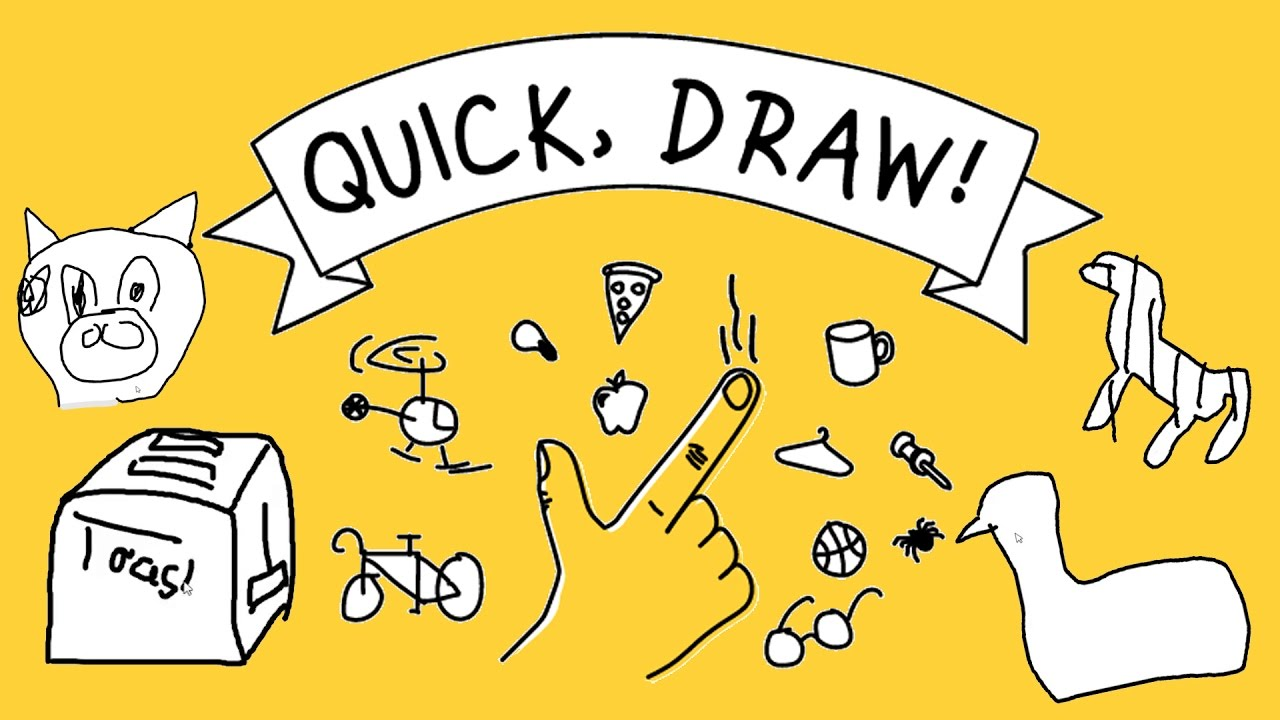
\includegraphics[width=1.0\linewidth]{Chapter2/Quick,_Draw!.jpg}
    \caption{Quick, Draw! by Google}
    \label{fig:baitoan}
\end{figure}

\section{Giải thích phần xử lý dữ liệu, giới thiệu mô hình, giải thích mô hình}

\subsection{Xây dựng tập dữ liệu} \label{sec:subsection221}

Quick,Draw thu thập dữ liệu thông qua việc yêu cầu người dùng vẽ các đồ vật cụ thể, chẳng hạn như "ngôi sao", "lá cây", "tia chớp", v.v. Dữ liệu được thu thập trong những lần vẽ của người dùng thông qua giao diện vẽ trực tuyến, và mỗi bản vẽ sẽ được gán nhãn dựa trên tên đồ vật mà người dùng đang vẽ.

\begin{figure}[H]  % H: Đặt hình ảnh ở vị trí chính xác
    \centering
    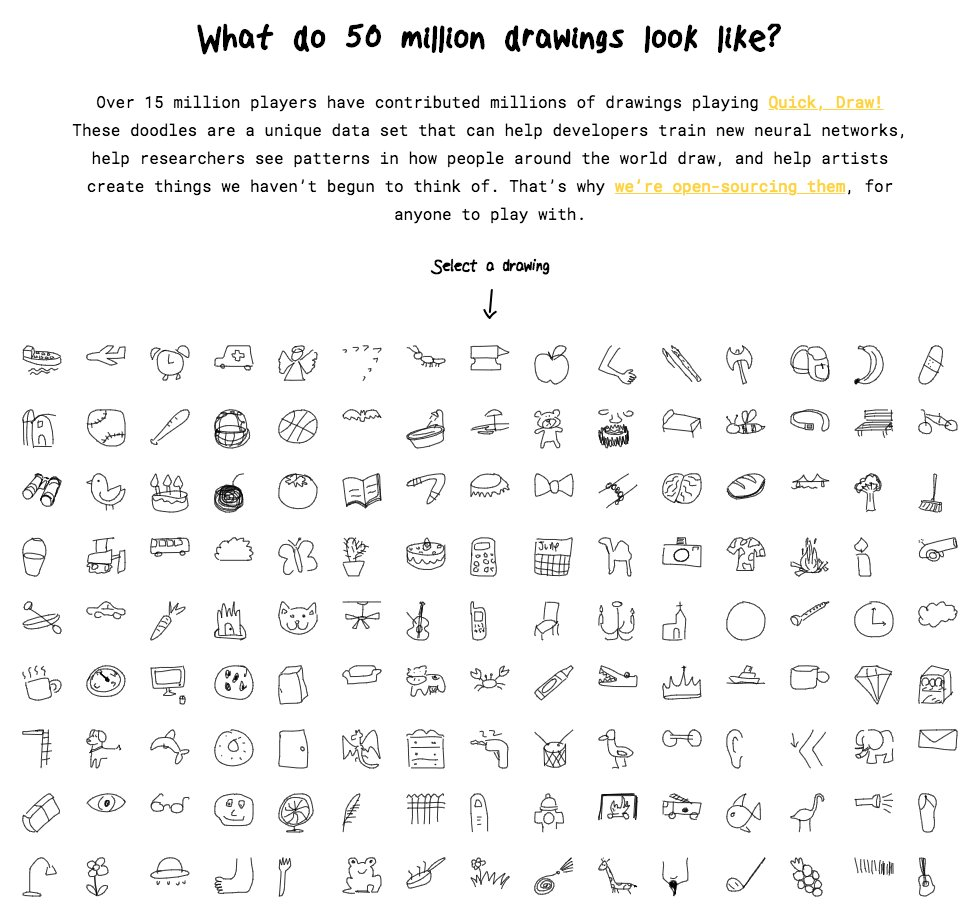
\includegraphics[width=0.75\linewidth]{Chapter2/QD_data.jpg}
    \caption{Xây dựng tập dữ liệu}
    \label{fig:baitoan}
\end{figure}

Dữ liệu vẽ ~\cite{DataSet} được thu thập từ hàng triệu người dùng trên toàn thế giới, với mỗi người vẽ một đối tượng trong một khoảng thời gian cố định (thường là 20 giây). Những bản vẽ này được ghi lại dưới dạng tọa độ của các điểm vẽ, từ đó có thể tạo ra một đường đi hoặc hình dạng của đồ vật.

Chúng ta sẽ sử dụng dữ liệu đã được Google chuẩn bị sẵn, là những bộ dữ liệu đã trải qua quá trình tiền xử lý cẩn thận. Dữ liệu này đã được chuẩn hóa tọa độ, chuyển đổi thành các vector đặc trưng, và được biểu diễn dưới dạng ma trận, đảm bảo tính đồng nhất và sẵn sàng cho quá trình huấn luyện. Thay vì tự tay thực hiện tất cả các bước tiền xử lý phức tạp, chúng ta sẽ tải trực tiếp dữ liệu đã được xử lý sẵn từ liên kết mà Google cung cấp. Điều này giúp tiết kiệm thời gian và tài nguyên, đồng thời đảm bảo rằng dữ liệu đầu vào của chúng ta luôn đạt chất lượng cao, hoàn hảo cho việc huấn luyện các mô hình học máy.

Sau khi chuẩn bị xong, chúng ta sẽ tiến hành phân chia dữ liệu theo tỷ lệ 80:20, với 80\% dùng cho việc huấn luyện mô hình và 20\% còn lại dành cho việc kiểm tra và đánh giá hiệu quả của mô hình. Đồng thời, chúng ta cũng sẽ mã hóa nhãn để đơn giản hóa quá trình xử lý, ví dụ như gán số 0 cho 'quả táo' và số 1 cho 'cuốn sách'. Việc mã hóa nhãn giúp mô hình dễ dàng nhận diện và phân loại các đối tượng, đồng thời tạo sự thuận tiện trong việc huấn luyện và đánh giá kết quả.

\subsection{Giới thiệu Mô hình}

Đoạn mã bạn đưa ra là một mô hình \textbf{QuickDraw} ~\cite{kaggle} được xây dựng bằng PyTorch, sử dụng kiến trúc \textbf{Convolutional Neural Network (CNN)} để giải quyết bài toán phân loại hình vẽ tay. Mô hình này bao gồm các lớp \textbf{Convolutional Layers (Conv2d), Fully Connected Layers (Linear)}, và các lớp \textbf{Dropout} để tránh overfitting.

\subsubsection{CNN là gì?}

Mạng nơ-ron tích chập (Convolutional Neural Networks - CNN) ~\cite{CNN}  là một trong những mô hình học sâu phổ biến nhất được sử dụng trong nhận dạng và phân loại hình ảnh. CNN đặc biệt hiệu quả trong việc nhận diện các đối tượng và nhận dạng khuôn mặt, hai lĩnh vực mà mô hình này được áp dụng rộng rãi. Với khả năng xử lý và phân tích các đặc trưng hình ảnh một cách tự động, CNN đã trở thành công cụ mạnh mẽ trong nhiều ứng dụng thực tế liên quan đến thị giác máy tính.

CNN phân loại hình ảnh bằng cách lấy 1 hình ảnh đầu vào, xử lý và phân loại nó theo các hạng mục nhất định (Ví dụ: Chó, Mèo, Hổ, ...). Máy tính coi hình ảnh đầu vào là 1 mảng pixel và nó phụ thuộc vào độ phân giải của hình ảnh. Dựa trên độ phân giải hình ảnh, máy tính sẽ thấy H x W x D (H: Chiều cao, W: Chiều rộng, D: Độ dày). Ví dụ: Hình ảnh là mảng ma trận RGB 6x6x3 (3 ở đây là giá trị RGB).

\begin{figure}[H]  % H: Đặt hình ảnh ở vị trí chính xác
    \centering
    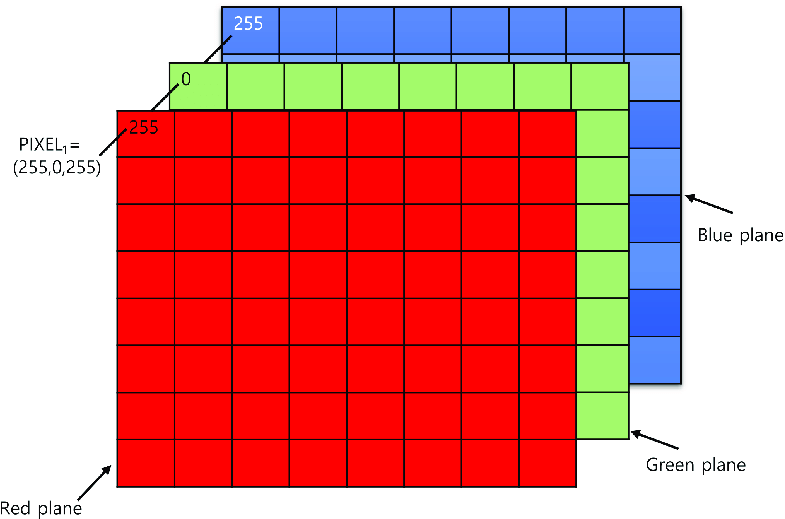
\includegraphics[width=0.75\linewidth]{Chapter2/RGB.png}
    \caption{RGB layers}
    \label{fig:baitoan}
\end{figure}

Về kỹ thuật, mô hình CNN để training và kiểm tra, mỗi hình ảnh đầu vào sẽ chuyển nó qua 1 loạt các lớp tích chập với các bộ lọc (Kernels), tổng hợp lại các lớp được kết nối đầy đủ (Fully Connected) và áp dụng hàm Softmax để phân loại đối tượng có giá trị xác suất giữa 0 và 1. Hình dưới đây là toàn bộ luồng CNN để xử lý hình ảnh đầu vào và phân loại các đối tượng dựa trên giá trị. 

\begin{figure}[H]  % H: Đặt hình ảnh ở vị trí chính xác
    \centering
    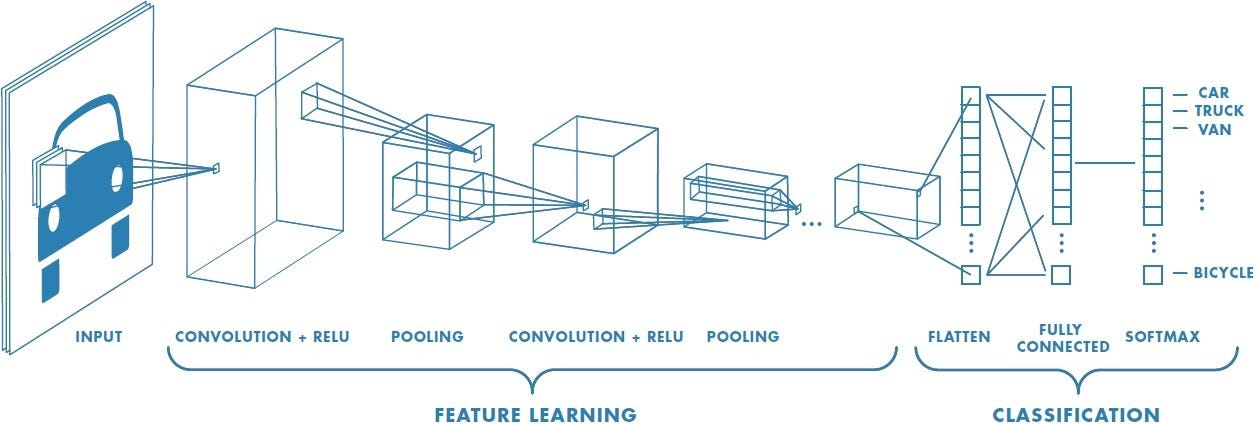
\includegraphics[width=0.75\linewidth]{Chapter2/CNN.jpg}
    \caption{Convolutional Neural Networks - CNN}
    \label{fig:baitoan}
\end{figure}

\subsubsection{Lớp tích chập - Convolution Layer}

Tích chập là lớp đầu tiên để trích xuất các tính năng từ hình ảnh đầu vào. Tích chập duy trì mối quan hệ giữa các pixel bằng cách tìm hiểu các tính năng hình ảnh bằng cách sử dụng các ô vuông nhỏ của dữ liệu đầu vào. Nó là 1 phép toán có 2 đầu vào như ma trận hình ảnh và 1 bộ lọc hoặc hạt nhân.

\begin{figure}[H]  % H: Đặt hình ảnh ở vị trí chính xác
    \centering
    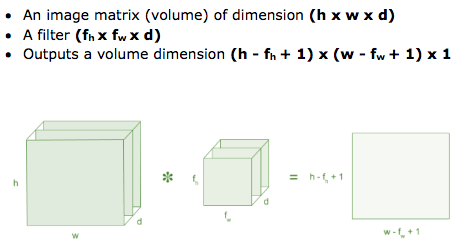
\includegraphics[width=0.75\linewidth]{Chapter2/CNN2.png}
    \label{fig:baitoan}
\end{figure}

Xem xét 1 ma trận 5 x 5 có giá trị pixel là 0 và 1. Ma trận bộ lọc 3 x 3 như hình bên dưới.

\begin{figure}[H]  % H: Đặt hình ảnh ở vị trí chính xác
    \centering
    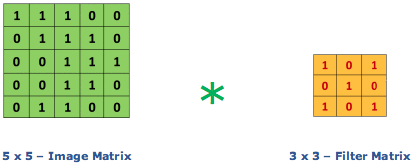
\includegraphics[width=0.75\linewidth]{Chapter2/CNN3.png}
    \label{fig:baitoan}
\end{figure}

Sau đó, lớp tích chập của ma trận hình ảnh 5 x 5 nhân với ma trận bộ lọc 3 x 3 gọi là 'Feature Map'

Sự kết hợp của 1 hình ảnh với các bộ lọc khác nhau có thể thực hiện các hoạt động như phát hiện cạnh, làm mờ và làm sắc nét bằng cách áp dụng các bộ lọc. Ví dụ dưới đây cho thấy hình ảnh tích chập khác nhau sau khi áp dụng các Kernel khác nhau.

\begin{figure}[H]  % H: Đặt hình ảnh ở vị trí chính xác
    \centering
    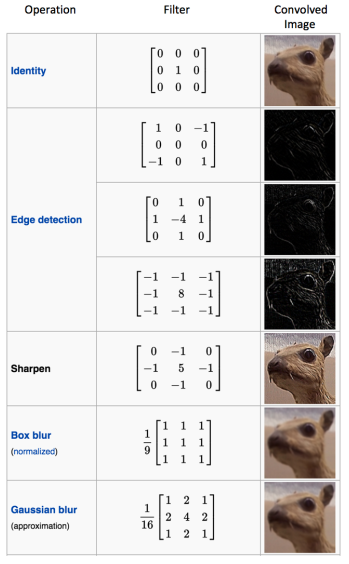
\includegraphics[width=0.75\linewidth]{Chapter2/CNN5.png}
    \label{fig:baitoan}
\end{figure}

\subsubsection{Hàm phi tuyến - ReLU}

ReLU viết tắt của Rectified Linear Unit, là 1 hàm phi tuyến. Với đầu ra là: ƒ (x) = max (0, x).

Tại sao ReLU lại quan trọng: ReLU giới thiệu tính phi tuyến trong ConvNet. Vì dữ liệu trong thế giới mà chúng ta tìm hiểu là các giá trị tuyến tính không âm.

\begin{figure}[H]  % H: Đặt hình ảnh ở vị trí chính xác
    \centering
    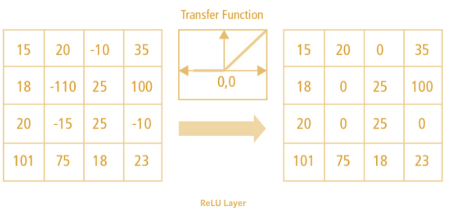
\includegraphics[width=0.75\linewidth]{Chapter2/RLU.png}
    \label{fig:baitoan}
\end{figure}

Có 1 số hàm phi tuyến khác như tanh, sigmoid cũng có thể được sử dụng thay cho ReLU. Hầu hết người ta thường dùng ReLU vì nó có hiệu suất tốt.

\subsubsection{Lớp gộp - Pooling Layer}

Lớp pooling sẽ giảm bớt số lượng tham số khi hình ảnh quá lớn. Không gian pooling còn được gọi là lấy mẫu con hoặc lấy mẫu xuống làm giảm kích thước của mỗi map nhưng vẫn giữ lại thông tin quan trọng. Các pooling có thể có nhiều loại khác nhau: Max Pooling, Average Pooling, Sum Pooling.

Max pooling lấy phần tử lớn nhất từ ma trận đối tượng, hoặc lấy tổng trung bình. Tổng tất cả các phần tử trong map gọi là sum pooling.

\begin{figure}[H]  % H: Đặt hình ảnh ở vị trí chính xác
    \centering
    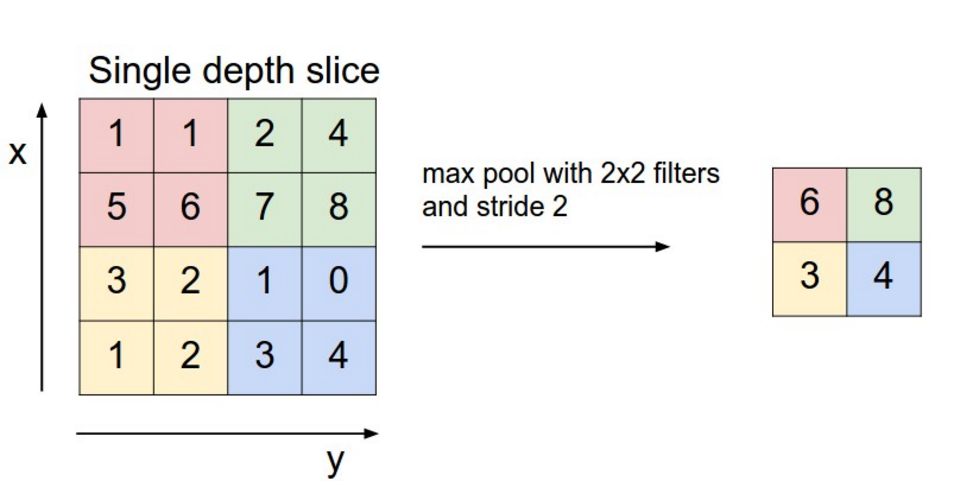
\includegraphics[width=0.75\linewidth]{Chapter2/Pooling.png}
    \label{fig:baitoan}
\end{figure}

\subsubsection{Dropout:}

Dropout là một kỹ thuật \textbf{regularization} (chuẩn hóa) được sử dụng để ngẫu nhiên loại bỏ (tắt) một số nơ-ron trong mạng nơ-ron trong quá trình huấn luyện. Khi sử dụng dropout, một tỷ lệ phần trăm của các nơ-ron trong mỗi lớp sẽ bị \textbf{tắt (drop)} ở mỗi lần huấn luyện, có nghĩa là những nơ-ron này không tham gia vào quá trình tính toán forward và không cập nhật trọng số trong quá trình backward.
\begin{enumerate}
    \item[-] \textbf{Cách hoạt động của Dropout}:
    \begin{itemize}
    \item \textbf{Trong quá trình huấn luyện}: Khi mạng nơ-ron được huấn luyện, dropout sẽ ngẫu nhiên loại bỏ một số nơ-ron khỏi mạng với xác suất nhất định, thường được gọi là tỷ lệ dropout. Ví dụ, nếu tỷ lệ dropout là 0.5, thì mỗi nơ-ron trong lớp sẽ có xác suất 50\% bị tắt đi trong mỗi lần cập nhật trọng số.
    \item \textbf{Trong quá trình dự đoán (inference)}: Khi mô hình đã được huấn luyện xong và thực hiện dự đoán trên dữ liệu mới, tất cả các nơ-ron sẽ được kích hoạt và sử dụng đầy đủ. Tuy nhiên, để bù đắp cho việc giảm số lượng nơ-ron trong quá trình huấn luyện, các trọng số của các nơ-ron được nhân với tỷ lệ giữ lại (1 - dropout rate).
    \end{itemize}
    \item[-] \textbf{Mục tiêu của Dropout}:
    \begin{itemize}
        \item \textbf{Giảm Overfitting}: Khi huấn luyện mạng nơ-ron, mô hình có thể dễ dàng "học thuộc" dữ liệu huấn luyện, tức là nó có thể ghi nhớ quá mức các đặc trưng cụ thể trong bộ dữ liệu và không thể tổng quát tốt khi gặp dữ liệu mới (dẫn đến overfitting). Dropout giúp giảm thiểu tình trạng này bằng cách ngăn mô hình phụ thuộc quá nhiều vào bất kỳ nơ-ron cụ thể nào, do đó tăng khả năng tổng quát của mô hình.
        \item \textbf{Tạo ra các mạng con ngẫu nhiên}: Dropout có tác dụng như một phương pháp tạo ra các "mạng con" ngẫu nhiên từ mạng lớn, giúp mô hình học được nhiều tính năng từ các đặc trưng khác nhau và không dựa vào những mối quan hệ quá chặt chẽ giữa các nơ-ron.
    \end{itemize}
\end{enumerate}

\subsection{Giải thích Mô hình}

\begin{enumerate}
    \item[] \textbf{Các phép toán trong mô hình}:
    
    \begin{itemize}
        \item \textbf{Convolution (CNN)}: Trong CNN, các lớp convolution giúp nhận diện các đặc trưng cơ bản của hình ảnh (như cạnh, góc, kết cấu) thông qua các bộ lọc (filters).
        \item \textbf{Activation function}: Các hàm kích hoạt (như ReLU, Sigmoid, Tanh) giúp thêm tính phi tuyến vào mô hình, từ đó cho phép mô hình học được các mối quan hệ phức tạp hơn.
        \item \textbf{Pooling layers (CNN)}: Giúp giảm kích thước đầu ra của các lớp convolution, tăng tính tổng quát và giảm sự phụ thuộc vào chi tiết không quan trọng.
        \item \textbf{LSTM/GRU (RNN)}: Các tế bào này giúp mô hình ghi nhớ thông tin trong các chuỗi thời gian dài hạn, nhờ vào cơ chế quên và ghi nhớ.
    \end{itemize}

\end{enumerate}

\subsubsection{Khởi tạo mô hình}

\begin{lstlisting}[language=python]
    def __init__(self, input_size=28, num_classes=15):
        super(QuickDraw, self).__init__()
\end{lstlisting}


\textcolor{blue}{\texttt{input\_size}}: Kích thước của hình ảnh đầu vào. Mặc định là 28, có nghĩa là hình ảnh đầu vào có kích thước 28x28 pixel (ví dụ như hình ảnh MNIST).

\textcolor{blue}{\texttt{num\_classes}}: Số lượng lớp phân loại đầu ra (mặc định là 15). Điều này có nghĩa là mô hình sẽ phân loại hình ảnh vào một trong 15 lớp.

\subsubsection{Quá trình huấn luyện}
\begin{enumerate}
    \item[\textbf{a.}] \textbf{Lớp Convolution đầu tiên (conv1):}

\begin{lstlisting}[language=python]
    self.conv1 = nn.Sequential(
        nn.Conv2d(1, 32, 5, bias=False),
        nn.ReLU(inplace=True),
        nn.MaxPool2d(2, 2)
    )
\end{lstlisting}


\begin{itemize}
    \item \textcolor{blue}{\texttt{nn.Conv2d(1, 32, 5, bias=False)}}: Đây là một lớp \textbf{convolution} 2D.
    \begin{itemize}
        \item \textcolor{blue}{\texttt{1}}: Số kênh đầu vào (1 kênh, tức là hình ảnh đen trắng).
        \item \textcolor{blue}{\texttt{32}}: Số kênh đầu ra (số lượng bộ lọc, nghĩa là 32 bộ lọc sẽ được áp dụng để trích xuất các đặc trưng từ hình ảnh).
        \item \textcolor{blue}{\texttt{5}}: Kích thước của kernel (lọc), tức là mỗi bộ lọc sẽ có kích thước 5x5.
        \item \textcolor{blue}{\texttt{bias=False}}: Không sử dụng thông số bias trong phép tính.
    \end{itemize}

    \item \textcolor{blue}{\texttt{nn.ReLU(inplace=True)}}: Hàm kích hoạt \textbf{ReLU} (Rectified Linear Unit), giúp thêm tính phi tuyến vào mô hình. \textcolor{blue}{\texttt{inplace=True}} có nghĩa là các phép toán sẽ được thực hiện trực tiếp trên tensor đầu vào mà không tạo ra bản sao mới.

    \item \textcolor{blue}{\texttt{nn.MaxPool2d(2, 2)}}: Lớp \textbf{MaxPooling} 2D, giúp giảm kích thước không gian của đầu ra từ lớp convolution.
    \begin{itemize}
        \item \textcolor{blue}{\texttt{2, 2}} có nghĩa là pooling sẽ lấy giá trị tối đa từ mỗi khu vực 2x2 của ma trận đầu vào, làm giảm chiều rộng và chiều cao của bản đồ đặc trưng xuống một nửa.
    \end{itemize}
\end{itemize}

\item[\textbf{b.}] \textbf{Lớp Convolution thứ hai (conv2):}

\begin{lstlisting}[language=python]
    self.conv2 = nn.Sequential(
        nn.Conv2d(32, 64, 5, bias=False),
        nn.ReLU(inplace=True),
        nn.MaxPool2d(2, 2)
    )
\end{lstlisting}

    \begin{itemize}
        \item \textcolor{blue}{\texttt{nn.Conv2d(32, 64, 5, bias=False)}}: Lớp convolution thứ hai. Sau lớp \textcolor{blue}{\texttt{conv1}}, đầu vào của lớp này có 32 kênh (từ 32 bộ lọc), và lớp này sẽ áp dụng 64 bộ lọc để trích xuất các đặc trưng cao hơn.
        
        \item Các tham số khác tương tự như lớp đầu tiên.

        \item \textcolor{blue}{\texttt{nn.ReLU(inplace=True) và nn.MaxPool2d(2, 2)}} vẫn giữ nguyên tác dụng như lớp đầu tiên, tạo tính phi tuyến và giảm kích thước đặc trưng.
    \end{itemize}
\end{enumerate}
\subsubsection{Lớp Fully Connected:}

\begin{lstlisting}[language=python]
    dimension = int(64 * pow(input_size/4 - 3, 2))
    self.fc1 = nn.Sequential(
        nn.Linear(dimension, 512),
        nn.Dropout(0.5)
    )
\end{lstlisting}

\begin{itemize}
    \item \textcolor{blue}{\texttt{dimension}}: Tính toán kích thước của đầu vào cho lớp \textcolor{blue}{\texttt{fc1}} (fully connected layer). Sau hai lần pooling (mỗi lần giảm kích thước của hình ảnh xuống một nửa), chiều rộng và chiều cao của hình ảnh sẽ bị giảm xuống còn một phần tư của kích thước ban đầu. Sau đó, chiều dài của đầu vào sẽ được tính bằng cách lấy số lượng kênh đầu ra của lớp \textcolor{blue}{\texttt{conv2}} (64) nhân với diện tích của bản đồ đặc trưng (chiều cao và chiều rộng).
    
    \begin{itemize}
        \item \textcolor{blue}{\texttt{input\_size / 4 - 3}}: Sau hai lần pooling, chiều cao và chiều rộng của hình ảnh giảm xuống một nửa mỗi lần. Sau đó, trừ đi 3 vì mỗi lớp convolution có kernel 5x5 và lớp pooling 2x2 làm giảm thêm chiều kích thước.
    \end{itemize}
    
    \item \textcolor{blue}{\texttt{nn.Linear(dimension, 512)}}: Lớp \textbf{fully connected} (mạng nơ-ron đầy đủ) đầu tiên, có 512 neuron. Đây là lớp dùng để kết nối các đặc trưng trích xuất từ các lớp convolution với các lớp đầu ra.

    \begin{itemize}
        \item \textcolor{blue}{\texttt{dimension}}: Số lượng đặc trưng đầu vào cho lớp này (được tính ở trên).
        \item \textcolor{blue}{\texttt{512}}: Số lượng neuron trong lớp \textcolor{blue}{\texttt{fc1}}.
    \end{itemize}
    
    \item \textcolor{blue}{\texttt{nn.Dropout(0.5)}}: Lớp \textbf{Dropout} được sử dụng để giảm overfitting. Trong quá trình huấn luyện, nó sẽ "tắt" ngẫu nhiên 50\% (tỷ lệ dropout là 0.5) của các neuron trong lớp này, giúp mô hình không quá phụ thuộc vào một số đặc trưng nhất định.

\end{itemize}

\begin{itemize}

\item[\textbf{c.}] \textbf{Lớp Fully Connected thứ hai (fc2):}

\begin{lstlisting}[language=python]
    self.fc2 = nn.Sequential(
        nn.Linear(512, 128),
        nn.Dropout(0.5)
    )
\end{lstlisting}

\begin{itemize}
    \item \textcolor{blue}{\texttt{nn.Linear(512, 128)}}: Lớp \textbf{fully connected} thứ hai, với 128 neuron. Đầu vào của lớp này là 512 đặc trưng từ lớp \textcolor{blue}{\texttt{fc1}}.
    \item \textcolor{blue}{\texttt{nn.Dropout(0.5)}}: Giống như lớp trước, lớp Dropout giúp giảm overfitting.
\end{itemize}

\item[\textbf{d.}] \textbf{Lớp Fully Connected cuối cùng (fc3):}

\begin{lstlisting}[language=python]
    self.fc3 = nn.Sequential(
        nn.Linear(128, num_classes)
    )
\end{lstlisting}

\begin{itemize}
    \item \textcolor{blue}{\texttt{nn.Linear(128, num\_classes)}}: Lớp \textbf{fully connected} cuối cùng để tạo ra đầu ra. Số lượng neuron trong lớp này là \textcolor{blue}{\texttt{num\_classes}}, tương ứng với số lượng lớp cần phân loại (ví dụ, nếu \textcolor{blue}{\texttt{num\_classes}} = 15, đầu ra sẽ là 15 giá trị).
\end{itemize}

\end{itemize}
    
\subsubsection{Hàm forward:}

\begin{lstlisting}[language=python]
    def forward(self, input):
        output = self.conv1(input)
        output = self.conv2(output)
        output = output.view(output.size(0), -1)
        output = self.fc1(output)
        output = self.fc2(output)
        output = self.fc3(output)
        return output
\end{lstlisting}

\begin{itemize}
    \item \textcolor{blue}{\texttt{self.conv1(input) và self.conv2(output)}}: Dữ liệu đầu vào sẽ đi qua các lớp convolutional (conv1 và conv2) để trích xuất các đặc trưng từ hình ảnh.
    \item \textcolor{blue}{\texttt{self.conv1(input) và self.conv2(output)}}: Dữ liệu đầu vào sẽ đi qua các lớp convolutional (conv1 và conv2) để trích xuất các đặc trưng từ hình ảnh.
    \item \textcolor{blue}{\texttt{output.view(output.size(0), -1)}}: Sau khi qua các lớp convolutional, dữ liệu có dạng (batch\_size, số kênh, chiều cao, chiều rộng). Dòng này sẽ làm phẳng (flatten) đặc trưng để đưa chúng vào các lớp fully connected. \textcolor{blue}{\texttt{output.size(0)}} là kích thước batch, và \textcolor{blue}{\texttt{-1}} giúp PyTorch tự động tính toán chiều còn lại.
    \item \textcolor{blue}{\texttt{self.fc1, self.fc2, self.fc3}}: Dữ liệu sau khi được làm phẳng sẽ đi qua các lớp fully connected để tạo ra đầu ra cuối cùng.
\end{itemize}

\subsection{Cách thức hoạt động:}

\begin{itemize}
    \item \textbf{Thư viện OpenCV}
    
    \begin{itemize}
        \textbf{OpenCV (Open Source Computer Vision Library)} là một thư viện mã nguồn mở mạnh mẽ và phổ biến được sử dụng để xử lý ảnh và video trong các ứng dụng thị giác máy tính. Thư viện này cung cấp một loạt các công cụ và thuật toán để thực hiện các nhiệm vụ như nhận diện đối tượng, phân tích hình ảnh, nhận dạng khuôn mặt, xử lý video, và nhiều ứng dụng khác liên quan đến thị giác máy tính.
    \end{itemize}

    \begin{figure}[H]  % H: Đặt hình ảnh ở vị trí chính xác
    \centering
    
\includegraphics[width=0.75\linewidth]{Chapter2/OpenCV-la-gi-1.jpeg}
    \caption{Logo OpenCV ~\cite{image}}
    \label{fig:baitoan}
    \end{figure}

    \item \textbf{Thư viện MediaPipe}:

    \begin{itemize}
         \textbf{MediaPipe} là một thư viện mã nguồn mở được phát triển bởi Google, chuyên cung cấp các công cụ và thuật toán mạnh mẽ để xử lý và phân tích hình ảnh, video, âm thanh trong thời gian thực. \textbf{MediaPipe} chủ yếu được thiết kế để xây dựng các ứng dụng và mô hình thị giác máy tính, học máy, và các tác vụ nhận dạng, phân tích hình ảnh/video với hiệu suất cao và đáp ứng thời gian thực.
    \end{itemize}

    \item \textbf{Thư viện hand}:

    \begin{itemize}
        \textbf{Hand} là một thư viện trong \textbf{MediaPipe} được phát triển để nhận diện và theo dõi các cử chỉ của bàn tay trong thời gian thực. Thư viện này giúp phát hiện và theo dõi các điểm đặc trưng của bàn tay, với mục tiêu phục vụ cho các ứng dụng như giao diện người dùng không chạm, thực tế tăng cường (AR), và các hệ thống nhận diện cử chỉ.
    \end{itemize}

    \item \textbf{Cách thức vẽ}

\begin{itemize}
    \item \textbf{Bằng camera\_app:}

    \begin{itemize}
        \item Để nhận diện các vật thể có màu đỏ làm trung tâm, ta sẽ sử dụng màu sắc đặc trưng này để xác định vị trí và nét vẽ của người dùng. Quá trình này sẽ bắt đầu bằng việc xác định các vật thể có màu đỏ trong khung hình, từ đó xác định vùng vẽ mà người dùng sẽ thực hiện. Khi người dùng bắt đầu vẽ, họ chỉ cần nhấn phím \textbf{backspace} để khởi động quá trình vẽ, hệ thống sẽ nhận diện và theo dõi các nét vẽ trong thời gian thực. Sau khi hoàn tất việc vẽ, người dùng sẽ tiếp tục nhấn lại phím \textbf{backspace} để kết thúc quá trình vẽ.

        \item Khi việc vẽ đã được hoàn tất và người dùng nhấn \textbf{backspace}, hệ thống sẽ sử dụng các nét vẽ đã được xác định để chuyển sang giai đoạn dự đoán. Lúc này, mô hình sẽ phân tích các nét vẽ và tiến hành dự đoán kết quả dựa trên các thông tin đã được thu thập. Phương pháp này giúp tạo ra một quá trình đơn giản và mượt mà, nơi người dùng chỉ cần thao tác cơ bản để tương tác với hệ thống, đồng thời giảm thiểu sự phức tạp trong việc sử dụng và điều khiển phần mềm.

        \item Khi người dùng muốn kết thúc chương trình, họ chỉ cần nhấn phím \textbf{Esc} để thoát khỏi ứng dụng. Việc này giúp đơn giản hóa quá trình đóng chương trình, không cần phải thực hiện nhiều thao tác phức tạp, chỉ cần một cú nhấn phím duy nhất để chương trình dừng lại và thoát hoàn toàn.
    \end{itemize}
    \item \textbf{Bằng Hand\_app:}

    \begin{itemize}
        \item Bằng cách sử dụng thư viện \textbf{Hand} để nhận diện các khớp tay của con người, chúng ta có thể tận dụng những chuyển động và vị trí của các ngón tay để tạo ra các nét vẽ. Cụ thể, khi người dùng giơ ngón trỏ lên và các ngón tay còn lại chụm lại, hệ thống sẽ nhận diện hành động này như là việc cầm cây bút. Khi người dùng di chuyển ngón trỏ, hệ thống sẽ hiểu đó là hành động vẽ, và các nét vẽ sẽ được tạo ra tương ứng với chuyển động của ngón tay.

    \begin{figure}[H]  % H: Đặt hình ảnh ở vị trí chính xác
    \centering
    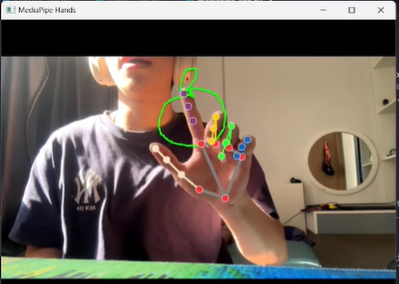
\includegraphics[width=0.75\linewidth]{Chapter2/Capture.PNG}
    \caption{Hand_drawing}

    \end{figure}
    
        \item Khi người dùng hoàn tất việc vẽ và muốn máy bắt đầu dự đoán kết quả, chỉ cần dang tay ra, mở rộng các ngón tay, và hệ thống sẽ nhận diện điều này như một dấu hiệu để kết thúc quá trình vẽ và chuyển sang giai đoạn dự đoán. Cách thức này giúp tạo ra một tương tác tự nhiên và mượt mà giữa người dùng và hệ thống mà không cần sử dụng bất kỳ thiết bị ngoại vi nào.

        \item Khi bạn muốn thoát khỏi chương trình, chỉ cần nhấn phím \textbf{Esc}.

    \end{itemize}
    
    \item \textbf{Bằng drawing\_app:}

    \begin{itemize}
        \item Bạn có thể sử dụng chuột để trực tiếp làm công cụ vẽ. Khi bắt đầu, chỉ cần nhấn phím \textbf{backspace} và bắt đầu vẽ trên bức tranh của mình. Khi hoàn tất việc vẽ và muốn hệ thống dự đoán, bạn chỉ cần nhấn lại phím \textbf{backspace} để kích hoạt quá trình dự đoán. Tương tự, để thoát khỏi chương trình, bạn chỉ cần nhấn phím \textbf{Esc}, giúp kết thúc ứng dụng một cách nhanh chóng và dễ dàng.
    \end{itemize}

\end{itemize}

\section{Experiment}

%Những qui định dưới này các bạn có thể bỏ qua hoặc đọc để hiểu thêm.
%Những định dạng này LaTeX đều tự động giúp các bạn.
%Các bạn xem hướng dẫn chi tiết hơn ở chương sau.

\subsection{ Giới thiệu dataset, mô tả dataset( gồm bao nhiêu mẫu, có những gì trong dataset)}

    Dữ liệu của Quickdraw ~\cite{experiment} được thu thập từ một nguồn do Google cung cấp, nơi mà người dùng trực tiếp vẽ các hình ảnh dựa trên các chủ đề đã được xác định trước. Những hình ảnh này không chỉ phản ánh khả năng vẽ của người dùng mà còn chứa đựng thông tin về cách thức mỗi cá nhân thể hiện một ý tưởng hoặc một đối tượng qua nét vẽ. Sau khi thu thập, các hình ảnh này được lưu trữ trong các tệp dữ liệu dưới dạng các mảng numpy (.npy), một định dạng phổ biến trong lĩnh vực học máy, giúp bảo toàn dữ liệu một cách hiệu quả và dễ dàng trong quá trình xử lý. Thay vì phải thu thập và chuẩn bị dữ liệu từ đầu, chúng ta có thể tận dụng các tệp dữ liệu này, được Google tạo sẵn, để thực hiện các nghiên cứu, phân tích hoặc xây dựng mô hình học máy mà không cần phải lo lắng về việc xử lý dữ liệu thô. Các tệp numpy chứa các mảng với thông tin hình ảnh đã được mã hóa sẵn, do đó chúng ta chỉ cần tải về và sử dụng chúng.

\begin{figure}[H]  % H: Đặt hình ảnh ở vị trí chính xác
\centering
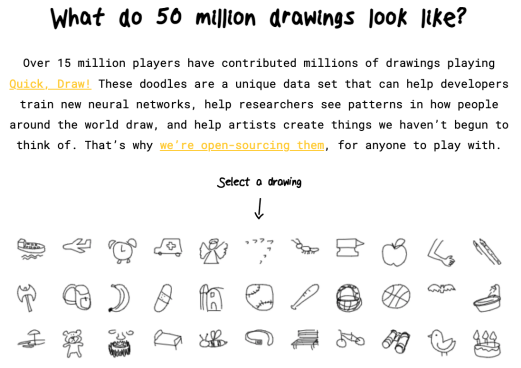
\includegraphics[width=0.75\linewidth]{Chapter2/QD2.png}
\caption{Quick, Draw! data}
\label{fig:baitoan}
\end{figure}

Vì giới hạn về dung lượng bộ nhớ và thời gian xử lý, chúng ta chỉ có thể sử dụng tối đa 20 bộ dữ liệu liên quan đến các đồ vật quen thuộc và dễ nhận diện trong đời sống hàng ngày. Những đồ vật này có thể bao gồm những hình ảnh đơn giản nhưng đầy tính biểu tượng như ngôi sao sáng rực trên bầu trời, chiếc lá cây mỏng manh đang đung đưa trong làn gió nhẹ, hay tia chớp lóe sáng rạch ngang bầu trời đen tối trong những cơn mưa giông. Mặc dù chỉ có 20 bộ dữ liệu, nhưng mỗi bộ chứa đựng những đặc điểm nổi bật và dễ nhận diện, mang lại giá trị trong việc xử lý và phân tích hình ảnh.

Việc lựa chọn những đồ vật quen thuộc này không chỉ giúp giảm thiểu độ phức tạp của bài toán mà còn tối ưu hóa khả năng tính toán, giúp tiết kiệm thời gian và tài nguyên trong quá trình thực hiện. Điều này đặc biệt quan trọng trong môi trường có giới hạn về dung lượng bộ nhớ hoặc khi thời gian xử lý là yếu tố quyết định. Dẫu vậy, với số lượng dữ liệu hạn chế, những đồ vật này vẫn đủ để giúp chúng ta xây dựng các mô hình nhận diện hoặc phân loại cơ bản, đáp ứng yêu cầu của bài toán mà không gặp phải sự quá tải về tài nguyên.

\begin{figure}[H]  % H: Đặt hình ảnh ở vị trí chính xác
\centering
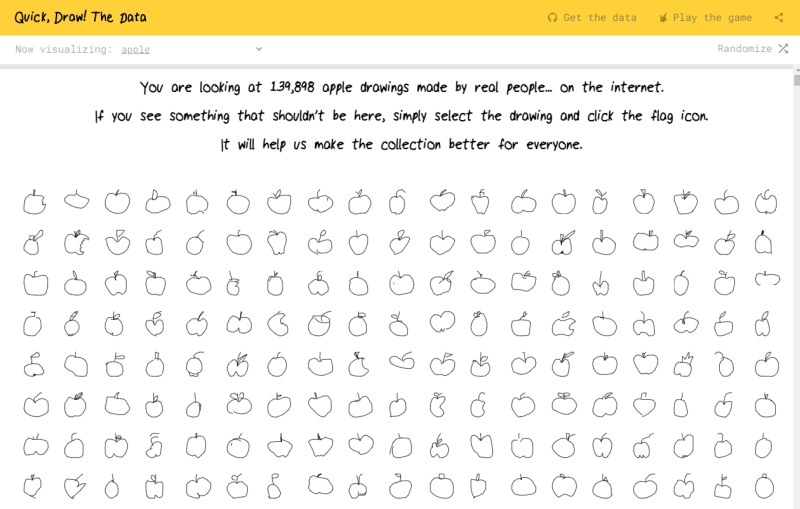
\includegraphics[width=0.75\linewidth]{Chapter2/QD1.png}
\label{fig:baitoan}
\end{figure}

\subsection{Cấu hình chạy thí nghiệm}

Để triển khai các bài toán nhận dạng và phân tích hình ảnh trong Python 3.6, chúng ta có thể sử dụng một số thư viện mạnh mẽ như \textbf{OpenCV (cv2), PyTorch, NumPy, Hand, và MediaPipe. OpenCV (cv2)} là thư viện phổ biến dùng để xử lý hình ảnh và video, với khả năng hỗ trợ nhận diện đối tượng, các phép biến đổi hình ảnh, cũng như các kỹ thuật xử lý ảnh thời gian thực. \textbf{PyTorch} là một thư viện học sâu mạnh mẽ, giúp xây dựng và huấn luyện các mô hình học máy, hỗ trợ tính toán tensor và GPU, rất phù hợp cho các tác vụ nhận dạng hình ảnh hoặc học sâu. \textbf{NumPy} là thư viện số học cơ bản, cung cấp các cấu trúc dữ liệu mảng mạnh mẽ và các phép toán số học hiệu quả, rất cần thiết khi làm việc với dữ liệu số hoặc hình ảnh. Hand và MediaPipe là hai thư viện đặc biệt mạnh trong việc xử lý và nhận dạng cử chỉ tay. MediaPipe cung cấp các mô hình đã được huấn luyện để phát hiện và theo dõi các điểm quan trọng trên tay người, trong khi Hand có thể hỗ trợ phân tích và nhận dạng các cử chỉ tay trong không gian 3D. Việc kết hợp các thư viện này tạo nên một cấu hình mạnh mẽ, hỗ trợ phát triển các ứng dụng nhận diện hình ảnh và phân tích cử chỉ tay, phục vụ cho các hệ thống nhận diện cử chỉ người dùng, tương tác bằng tay, và nhiều ứng dụng khác trong lĩnh vực thị giác máy tính.

\subsection{Kết quả chạy thí nghiệm}

Nhìn chung, mô hình ~\cite{github} có khả năng dự đoán khá chính xác khi nhận diện các vật thể đơn giản. Tuy nhiên, khi gặp những vật thể phức tạp hoặc khó nhận diện, mô hình vẫn gặp phải một số sai sót và nhầm lẫn trong việc dự đoán.

\begin{figure}[H]  % H: Đặt hình ảnh ở vị trí chính xác
\centering
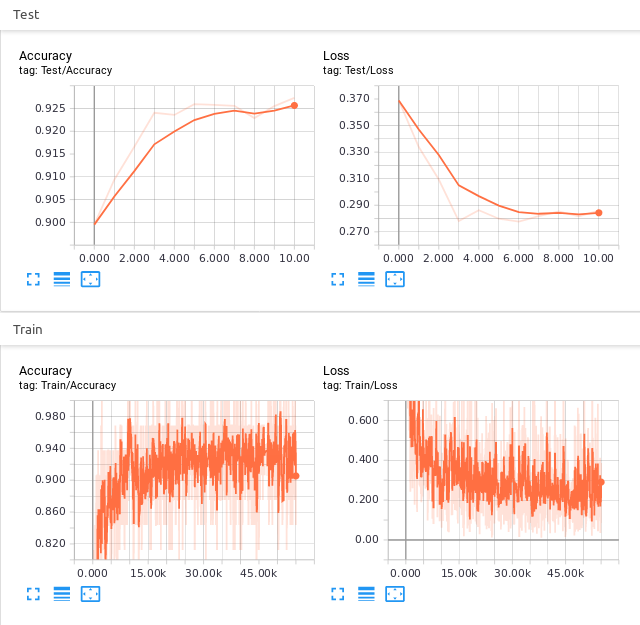
\includegraphics[width=0.75\linewidth]{Chapter2/Accuracy.png}
\label{fig:baitoan}
\end{figure}

\section{Kết luận}

Quick, Draw vẫn là một công cụ rất ấn tượng và thú vị, mang lại trải nghiệm giải trí hấp dẫn và hiệu quả trong việc giải tỏa căng thẳng. Mặc dù mô hình của nó khá đơn giản, nhưng sự cuốn hút từ cách thức người dùng tương tác và sự thú vị trong việc thử thách khả năng vẽ khiến nó trở thành một công cụ giải trí tuyệt vời. Với khả năng nhận diện hình ảnh dựa trên các nét vẽ đơn giản, Quick, Draw vẫn giữ được sự hấp dẫn và dễ tiếp cận, làm cho người dùng không thể rời mắt khỏi trò chơi này.

Mặc dù mô hình có thể đưa ra những dự đoán tương đối chính xác trong hầu hết các trường hợp, nhưng đôi khi kết quả dự đoán vẫn có thể bị sai lệch. Một trong những nguyên nhân chính của sự sai lệch này có thể là do chất lượng của các nét vẽ không được hoàn hảo. Người dùng có thể vẽ một cách vội vàng, không rõ ràng hoặc thậm chí là không đúng với hình dạng chuẩn mà mô hình đã được huấn luyện. Bên cạnh đó, các yếu tố khác như độ mờ của nét vẽ, sự khác biệt trong cách vẽ của từng người hay các biến thể trong cách thể hiện các đối tượng có thể gây khó khăn cho mô hình khi nhận diện và phân loại hình ảnh.

Ngoài ra, mặc dù bộ dữ liệu của Quickdraw bao gồm hàng trăm ngàn mẫu hình ảnh, nhưng không thể tránh khỏi sự tồn tại của một số sai sót, chẳng hạn như những nét vẽ sai hoặc không chính xác từ người dùng. Những sai sót này có thể xảy ra do nhiều yếu tố như người dùng vẽ vội, không chú ý, hoặc thiếu kỹ năng vẽ. Khi các dữ liệu này được sử dụng trong quá trình huấn luyện mô hình, chúng có thể gây ra một số sai lệch nhỏ trong kết quả dự đoán. Những "lỗi" này, dù là nhỏ, vẫn có thể ảnh hưởng đến độ chính xác của mô hình trong một số trường hợp. Tuy nhiên, đây là một vấn đề không thể hoàn toàn tránh khỏi khi làm việc với dữ liệu thực tế, đặc biệt khi dữ liệu được thu thập từ nhiều người dùng khác nhau với các mức độ kỹ năng vẽ và cách thể hiện rất khác nhau.


\chapter{Báo cáo làm việc hàng tuần}
\label{Chapter3}

\begin{enumerate}
    \section{Họp lần 1}
        \begin{enumerate}
            \item Ngày họp: 6/12/2024
            \item Thành viên tham dự:
                \begin{enumerate}
                    \item[-] Mai Hoàng Hiệp
                    \item[-] Trần Trung Hiếu
                    \item[-] Nguyễn Duy Đạt
                \end{enumerate}
            \item Phân công:
                \begin{enumerate}
                    \item[-] Nội dung phân công:
                    \begin{itemize}
                        \item cài đặt và chạy được mô hình sau khi tham khảo [1, 2, 3]
                        \item  up soucre code lên github [2]
                        \item làm nội dung ghi vào Latex và slide [1, 3]
                        \item làm báo cáo bằng Latex [3]
                        \item làm slide [1, 2, 3]
                        \item làm video thuyết trình [1, 2]
                    \end{itemize} 
                    \item[-] Thời gian làm: 7/12/2024 - 18/12/2024
                    \item[-] Người được phân công: 
                    \begin{itemize}
                        \item Mai Hoàng Hiệp [1], Trần Trung Hiếu [2], Nguyễn Duy Đạt [3]
                    \end{itemize}
                \end{enumerate}
            \item Tiến độ làm tuần trước:
                \begin{enumerate}
                    \item[-] Nội dung phân công: Không
                    \item[-] Người được phân công: Không
                    \item[-] Tiến độ làm: Mai Hoàng Hiệp đã tham khảo được các nguồn tài liệu, video hướng dẫn về Quick, Draw!.
                    \item[-] Công việc đã làm: tạo github của nhóm để up source code, tham khảo các tài liệu liên quan.
                    \item[-] Công việc chưa làm: training và chạy được mô hình, làm nội dung ghi vào Latex và Slide, làm báo cáo bằng Latex, làm slide thuyết trình, video thuyết trình + demo chương trình, up source code lên github.
                \end{enumerate}
        \end{enumerate}
    \section{Họp lần 2}
        \begin{enumerate}
            \item Ngày họp: 11/12/2024
            \item Thành viên tham dự:
                \begin{enumerate}
                    \item[-] Mai Hoàng Hiệp
                    \item[-] Trần Trung Hiếu
                    \item[-] Nguyễn Duy Đạt
                \end{enumerate}
            \item Phân công:
                \begin{enumerate}
                    \item[-] Nội dung phân công:
                    \begin{itemize}
                        \item đọc hiểu lại từng phần code [1, 2, 3]
                        \item hoàn thiện nội dung của báo cáo bằng Latex [1, 3]
                        \item làm slide thuyết trình [1, 2, 3]
                        \item làm video thuyết trình + demo chương trình [1, 2]
                    \end{itemize}
                    \item[-] Thời gian làm: 11/12/2024-18/12/2024
                    \item[-] Người được phân công:
                    \begin{itemize}
                        \item Mai Hoàng Hiệp [1], Trần Trung Hiếu [2], Nguyễn Duy Đạt [3]
                    \end{itemize}
                \end{enumerate}
            \item Tiến độ làm tuần trước:
                \begin{enumerate}
                    \item[-] Nội dung phân công: hoàn tất các bước của chương trình yêu cầu, hoàn thành quá trình training, viết tiếp báo cáo Latex, viết nội dung trình chiếu, làm video, làm slide, up source code lên github.
                    \item[-] Người được phân công: Mai Hoàng Hiệp, Trần Trung Hiếu, Nguyễn Duy Đạt. 
                    \item[-] Tiến độ làm: làm tiếp Latex, hoàn thành source code, hoàn thành quá trình training, chạy được mô hình hoạt động ổn định.
                    \item[-] Công việc đã làm: Nội dung thêm vào Latex (từ đầu đến chapter 1), source code up lên github. 
                    \item[-] Công việc chưa làm: Latex (các phần chapter 2, chapter 3 và references), slide thuyết trình, Video.
                \end{enumerate}
        \end{enumerate}
    \section{Họp lần 3}
        \begin{enumerate}
            \item Ngày họp: 17/12/2024
            \item Thành viên tham dự:
                \begin{enumerate}
                    \item[-] Mai Hoàng Hiệp
                    \item[-] Trần Trung Hiếu
                    \item[-] Nguyễn Duy Đạt
                \end{enumerate}
            \item Phân công:
                \begin{enumerate}
                    \item[-] Nội dung phân công:
                    \begin{itemize}
                        \item Làm video thuyết trình bằng cách ghi âm chèn vào slide [1, 2, 3]
                        \item hoàn thiện slide [1, 3]
                        \item hoàn thiện Latex [2, 3]
                    \end{itemize}
                    \item[-] Thời gian làm: 17/12/2024 - 18/12/2024
                    \item[-] Người được phân công:
                    \begin{itemize}
                        \item Mai Hoàng Hiệp [1], Trần Trung Hiếu [2], Nguyễn Duy Đạt [3]
                    \end{itemize}
                \end{enumerate}
            \item Tiến độ làm tuần trước:
                \begin{enumerate}
                    \item[-] Nội dung phân công: hoàn thiện source code, hoàn thiện Latex, Slide, Video.
                    \item[-] Người được phân công: Mai Hoàng Hiệp, Trần Trung Hiếu, Nguyễn Duy Đạt.
                    \item[-] Tiến độ làm: đang làm tiếp Latex, hoàn thiện slide thuyết trình.
                    \item[-] Công việc đã làm: Latex (chapter 2 và references), source code, slide.
                    \item[-] Công việc chưa làm: Video, Latex (chapter 3).
                \end{enumerate}
        \end{enumerate}
\end{enumerate}

% Công trình của tác giả (nếu không có thì comment 02 dòng dưới)
% \addcontentsline{toc}{chapter}{Danh mục công trình của tác giả}
% \chapter*{Danh mục công trình của tác giả}
\label{Appendix1}

\begin{enumerate}
\item Tạp chí ABC
\item Tạp chí XYZ
\end{enumerate}

% In tài liệu tham khảo
% In tài liệu tham khảo
\addcontentsline{toc}{chapter}{Tài liệu tham khảo}
\printbibheading[title={Tài liệu tham khảo}]

\printbibliography[heading=subbibliography, title={Tiếng Việt}, keyword=Viet, resetnumbers=true]

\DeclareNameAlias{sortname}{last-first}
\DeclareNameAlias{default}{last-first}

\printbibliography[heading=subbibliography, title={References}]
% ===================================================================== %
% CHÚ Ý: phải gán lại resetnumbers=số tài liệu tham khảo tiếng Việt + 1 %
% ===================================================================== %

% Phần phụ lục
% \appendix

\chapter{Ngữ pháp tiếng Việt}
\label{Appendix1}

Đây là phụ lục.
% \chapter{Ngữ pháp tiếng Nôm}
\label{Appendix2}

Đây là phụ lục 2.

\end{document} 